\documentclass{thesisclass}

%% Bibstyle %%
\usepackage[numbers]{natbib}

\usepackage{float}
\usepackage{multirow}
\usepackage{listings}
\usepackage{placeins}
\usepackage{graphicx}
% My OWN PACKAGE %
%\usepackage[latin1]{inputenc}%
\graphicspath{ {images/} }

%% Glossar %%
\usepackage[toc,nonumberlist]{glossaries}
\makeglossaries

\lstset{language=Java,
   basicstyle=\small,
   keywordstyle=\color{blue!80!black!100},
   identifierstyle=,
   commentstyle=\color{green!50!black!100},
   stringstyle=\ttfamily,
   breaklines=true,
   %numbers=left,
   numberstyle=\small,
   %frame=single,
   backgroundcolor=\color{blue!3}
} 
\renewcommand*{\lstlistingname}{Quelltextausschnitt}


% Based on thesisclass.cls of Timo Rohrberg, 2009
% ----------------------------------------------------------------
% Thesis - Main document
% ----------------------------------------------------------------

%% ---------------------------------
%% | Information about the thesis  |
%% ---------------------------------

\newcommand{\myname}{Weinmann Philipp}
\newcommand{\mytitle}{Maschinelles Lernen im Kontext der Programmierung natürlicher Sprachen}
\newcommand{\myinstitute}{Institut f\"ur Programmstrukturen\\
											und Datenorganisation (IPD)}
											
\newcommand{\advisor}{Dipl. Inform. Alexander Wachtel}

%\newcommand{\timestart}{Startdatum}
%\newcommand{\timeend}{Enddatum}
\newcommand{\submissiontime}{[FILL OUT DATE HERE]}


%% -------------------------------
%% |  Information for PDF file   |
%% -------------------------------
\hypersetup{
 pdfauthor={\myname},
 pdftitle={\mytitle},
 pdfsubject={Not set},
 pdfkeywords={Not set}
}

%%%%%%%%%%%%%%%%%%%%%%%%%%%%%%%%%
%% Here, main documents begins %%
%%%%%%%%%%%%%%%%%%%%%%%%%%%%%%%%%
\begin{document}

% Describe separation hints here:
%% --------------------------------
%% | Settings for word separation |
%% --------------------------------
% Help for separation:
% In german package the following hints are additionally available:
% "- = Additional separation
% "| = Suppress ligation and possible separation (e.g. Schaf"|fell)
% "~ = Hyphenation without separation (e.g. bergauf und "~ab)
% "= = Hyphenation with separation before and after
% "" = Separation without a hyphenation (e.g. und/""oder)

\hyphenation{
Sprach-ein-ga-ben
}

\selectlanguage{ngerman}
\floatname{algorithm}{Algorithmus}

\frontmatter
\pagenumbering{roman}
%% titlepage.tex
%%

% coordinates for the bg shape on the titlepage
\newcommand{\diameter}{20}
\newcommand{\xone}{-15}
\newcommand{\xtwo}{160}
\newcommand{\yone}{15}
\newcommand{\ytwo}{-253}

\begin{titlepage}
% bg shape
\begin{tikzpicture}[overlay]
\draw[color=gray]  
 		 (\xone mm, \yone mm)
  -- (\xtwo mm, \yone mm)
 arc (90:0:\diameter pt) 
  -- (\xtwo mm + \diameter pt , \ytwo mm) 
	-- (\xone mm + \diameter pt , \ytwo mm)
 arc (270:180:\diameter pt)
	-- (\xone mm, \yone mm);
\end{tikzpicture}
	\begin{textblock}{10}[0,0](4,2.5)
		
\includegraphics[width=.3\textwidth]{logos/KITLogo_RGB.pdf}
	\end{textblock}
	\changefont{phv}{m}{n}	% helvetica	
	\vspace*{3.5cm}
	\begin{center}
		\Huge{\mytitle}
		\vspace*{2cm}\\
		\Large{
			\iflanguage{english}{Seminar Paper of}			
												  {Seminararbeit \\von} 
		}\\
		\vspace*{1cm}
		\huge{\myname}\\
		\vspace*{1cm}
		\Large{
			\iflanguage{english}{At the Department of Informatics}			
													{An der Fakult\"at f\"ur Informatik}
			\\
			\myinstitute
		}
	\end{center}
	\vspace*{1cm}
\Large{
\begin{center}
\begin{tabular}[ht]{l c l}
  % Gutachter sind die Professoren, die die Arbeit bewerten. 
%  \iflanguage{english}{Reviewer}{Erstgutachter}: & \hfill  & \reviewerone\\
 % \iflanguage{english}{Second reviewer}{Zweitgutachter}: & \hfill  & \reviewertwo\\
  \iflanguage{english}{Advisor}{Betreuer}: & \hfill  & \advisor\\
 % \iflanguage{english}{Second advisor}{Zweiter Betreuer}: & \hfill  & \advisortwo\\
  % Der zweite betreuende Mitarbeiter kann weggelassen werden. 
\end{tabular}
\end{center}
}


%\vspace{2cm}
%\begin{center}
%\large{\iflanguage{english}{Duration:}{Bearbeitungszeit}: \timestart \hspace*{0.25cm} -- \hspace*{0.25cm} \timeend}
%\end{center}


\begin{textblock}{10}[0,0](4,16.8)
\tiny{ 
	\iflanguage{english}
		{KIT -- University of the State of Baden-Wuerttemberg and National Research Center of the Helmholtz Association}
		{KIT -- Universit\"at des Landes Baden-W\"urttemberg und nationales Forschungszentrum in der Helmholtz-Gemeinschaft}
}
\end{textblock}

\begin{textblock}{10}[0,0](14,16.75)
\large{
	\textbf{www.kit.edu} 
}
\end{textblock}

\end{titlepage}

\blankpage
\vspace*{36\baselineskip}
\hbox to \textwidth{\hrulefill}
\par
\iflanguage{english}{I declare that I have developed and written the enclosed thesis completely by myself, and have not used sources or means without declaration in the text.}{Ich versichere wahrheitsgem\"a\ss, die Arbeit selbstst\"andig angefertigt, alle benutzten Hilfsmittel vollst\"andig und genau angegeben und alles kenntlich gemacht zu haben, was aus Arbeiten anderer unver\"andert oder mit Ab\"anderungen entnommen wurde.}

\iflanguage{english}{I followed the rules for securing a good scientific pracise of the Karlsruhe Institute of Technology (Regeln zur Sicherung guter wissenschaftlicher Praxis im Karlsruher Institut f\"ur Technologie (KIT)).}{Die Regeln zur Sicherung guter wissenschaftlicher Praxis im Karlsruher Institut f\"ur Technologie (KIT) habe ich befolgt.}

\textbf{Karlsruhe, \submissiontime{}}
\vspace{1.5cm}

\dotfill\hspace*{8.0cm}\\
\hspace*{2cm}(\textbf{\myname{}}) %center name with hspace

\thispagestyle{empty}

\blankpage

%inspirational quote%
%vspace centers the quote horizontally%
\vspace*{\fill}
\begin{figure}[h]
  \center
  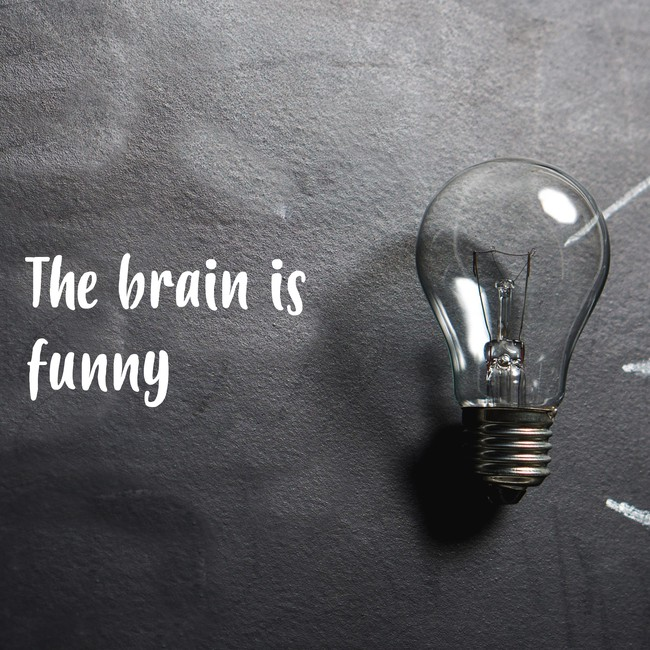
\includegraphics[width=250px]{images/inspirobotQuote.jpg}
  \caption{Quote generated through an AI \cite{inspirobot}}
  \label{fig:Inspirational quote by AI}
\end{figure}
\vspace*{\fill}\clearpage

%% -------------------
%% |   Directories   |
%% -------------------
\tableofcontents
\cleardoublepage

%\listoffigures
%
%\listoftables
%\cleardoublepage

% Glossary


\newglossaryentry{IA}{
	name=IA,
	description=Intelligenter (persönlicher) Assistent
}

\newglossaryentry{KI}{
	name=KI,
	description = Jegliches Programm\, das es einer Maschine erm\"oglicht auf ihre Umwelt zu reagieren.
}

\newglossaryentry{MaschinellesLernen}{
	name = ML,
	description = Maschinelles Lernen\, künstliche generierung von Wissen aus Erfahrung.
}

\newglossaryentry{ANN}{
	name = ANN,
	description = Artificial Neural Network\, ein Künstliches Neuronales Netz.
}

\newglossaryentry{FFN}{
	name = FFN,
	description = Feed Forward Network\, ein Künstliches Neuronales Netz dessen Neuronen einen Azyklischen Graph bilden.
}

\newglossaryentry{FCNN}{
	name = Fully connected Neural Network,
	description = ein Neuronales Netz\, in dem jede Lage mit der nächsten verbunden ist.
}

\newglossaryentry{RNN}{
	name = RNN,
	description = Recurrent Neural Network\, ein Neuronales Netz\, das im gegenzug zu Feed Forward Netzten es erlaubt Signale an vorangehende Schichten zurückzugeben.
}

\newglossaryentry{test}{
name = testosterone,
description = itworks
}

\newglossaryentry{MT}{
name = MT,
description = Machine Translation\, eine automatische Übersetzung von geschriebener oder gesprochener Sprache in eine andere Sprache bzw. Form.
} 

\newglossaryentry{NMT}{
name = NMT,
description = Neural machine translation\, automatische Übersetzung von geschriebener oder gesprochener Sprache in eine andere Sprache bzw. Form mithilfe von Künstlichen Neuronalen Netzen (ANN).
}

\newglossaryentry{NLP}{
name = NLP,
description = natural language programming\, Programmieren in natürlicher Sprache\, z.B Deutsch oder Englisch.
}

\newglossaryentry{Backpropagation}{
	name = Backpropagation,
	description = Ein Werkzeug das es ANN ermöglicht zu trainieren. Weights und Biases werden geupdated.
}

\newglossaryentry{Tensorflow}{
	name = Tensorflow,
	description = Ein Open Source Framework für ANN von Google.
}

\newglossaryentry{Ausreisser}{
	name = Ausreißer,
	description = Ein Funktionswert\, der um ein vielfaches von seinem zeitlich vorgehenden Wert abweicht.
}

\newglossaryentry{Turingtest}{
	name = Turingtest,
	description = ein von Alan Turing entwickelter Test\, ob eine Maschine ein dem Menschen gleichwertiges Denkvermögen hat
	}

%% -----------------
%% |   Main part   |
%% -----------------

%Abstract%
\chapter{Abstract}
[TODO] Ein Abstract ist eine prägnante Inhaltsangabe, ein Abriss ohne Interpretation und Wertung einer wissenschaftlichen Arbeit.
\newpage

\section{Was ist Maschinelles Lernen}

\begin{figure}[h!]
  \center
  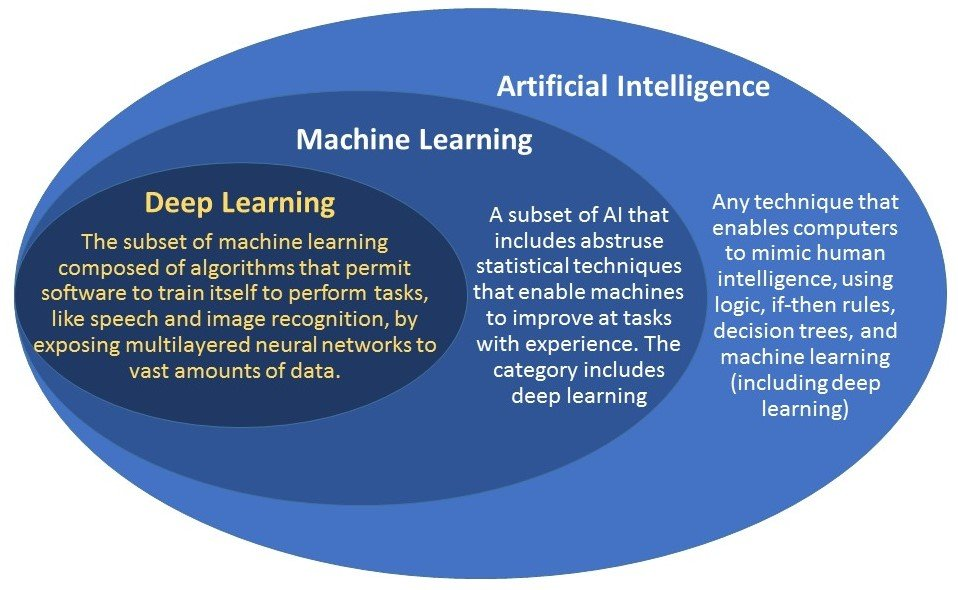
\includegraphics[width=\textwidth]{images/machineLearningInAI.jpg}
  \caption{Veranschaulichung, wie Maschinelles Lernen einzuordnen ist. \cite{machineLearning1}}
  \label{fig:Veranschaulichung, wie Maschinelles Lernen einzuordnen ist.}
\end{figure}

Maschinelles Lernen ist ein Teilbereich der Künstlichen Intelligenz. Es handelt sich also um eine Methode, die es Maschinen ermöglicht auf ihre Umwelt zu reagieren. Es ist jedoch oft schwierig wenn nicht unmöglich von Hand zu erkennen welche Reaktion das beste Ergebniss liefert, hier kommt Maschinelles Lernen ins Spiel. Dank statistischer Auswertungen können Algorithmen entstehen, die (meißtens) korrekte Ergebnisse liefern, ohne das der Programmierer sich Gedanken machen muss, wie der Algorithmus letzendlich aufgebaut ist. \newline
Während diese Methode der Datenauswertung schon lange bekannt ist  

\subsection{Anwendungen im Bereich der Informatik}
	In jedem Gebiet in dem große Mengen an Daten zur Verfügung stehen bzw. generiert werden können, ist Maschine Learning theoretisch anwendbar. Weil dies auf so ziemlich jeden Bereich der Informatik zutriff, wird so viel Hoffnung in diese Art von Algorithmen gesteckt. \newline
Obwohl die Theorie hinter dieser Art der Datenauswertung seit langem bekannt ist, so finden mächtigere Algorithmen die meißt auf Neuronalen Netzen basieren erst seit kurzem verbreitete Anwendung dank verbesserter Rechenleistung. [CITATION NEEDED?]\newline
	\newline Anwendungsbereiche sind zum Beispiel:
\begin{itemize}
	\item Gesichtserkennung
	\item Spamerkennung (Email)
	\item Spracherkennung
	\item automatische Medikamentenentwicklung
	\item Maschinelle Übersetzungen
\end{itemize}
In dieser Ausarbeitung werden wir uns insbesondere für Maschinelle Übersetzungen interessieren.

\section{Aufkommen von Maschinellem Lernen}
Maschinelles Lernen generell und insbesondere Neuronale Netze erfreuen sich seit einigen Jahren (stand 2018) großer Aufmerksamkeit. Der Grundstein für diese Verfahren wurde jedoch schon Ende des 18. Jahrhunderts von Thomas Bayes gelegt\cite{bayes1763essay}. \newline
Während die ersten Anwendungen zum Größteil (meißt abstrakter) mathematischer natur waren\cite{legendre1805nouvelles}, so befasst sich schon 1913 das erste Paper mit der Analyse von Gedichten\cite{markov2006example}. Dort analysiert Markov ein Gedicht und bemerkt, das man Wahrscheinlichkeiten formulieren kann, welche Eigenschaften weitere Teile vom Text haben ohne das man die Gesamtheit des Gedichtes in betracht ziehen muss. \newline
Ab der Zweiten hälfte des 20. Jahrhunderts wurden enddeckungen im bereich des Maschinellen Lernens gemacht, die heute jedem der mit dem fach zu tun hat bekannt sind. 1950 formuliert Alan Turing die Turing Learning Machine \cite{machinery1950computing}, ein Jahr später entwickeln und bauen zwei Wissenschaftler das erste Neuronale Netz\cite{snarc}. 1957 entwickelt Frank Rosenblatt den "perceptron"\cite{rosenblatt1958perceptron}, ein erstes Modell eines fully connected neural network.
%original draft of a perceptron from Frank Rosenblatt%
\begin{figure}[H]
  \center
  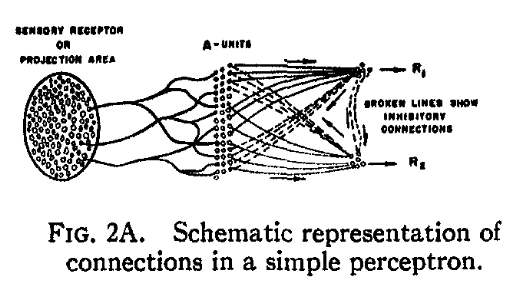
\includegraphics[width=\textwidth]{images/perceptron.png}
  \caption{original draft of a perceptron in the original paper}
  \label{fig:perceptron}
\end{figure}
Nachdem [CONTINUE HERE]

\section{Neuronale Netze}
	\subsection{Einführung}
		Ein technischer Durchbruch ist oft "nur" die gelungene Nachahmung eines in der Natur vorkommenden Phänomens. Neuronale Netze kann man Vergleichen mit dem Versuch das menschliche Gehirn nachzubauen.[CITATION?] Während diese Unterfangen nicht oder nur teilweise gelungen sind, haben sich einige Nebenprodukte dieser Forschung als sehr nützlich erwiesen.
Ein Neuronales Netz besteht aus Knoten die "künstliche Neuronen" genannt. Diese können auf verschiedene Weise miteinander verbunden sein. Diese Verbindungen werden oft "Synapsen" genannt. Jedes Neuron kann Signale empfangen und weiterleiten. Die Anzahl an Neuronen sowie die exakten Verbindungen bzw. die Information wann ein Signal mit welcher Stärke weitergeleitet wird stellt den Algorithmus dar.
\begin{figure}[h]
  		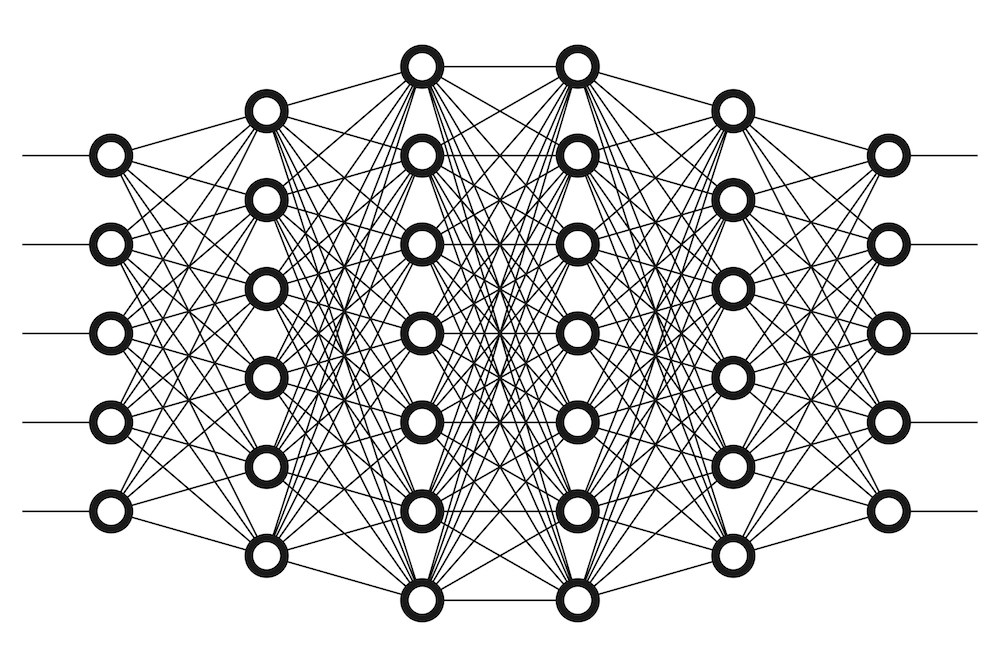
\includegraphics[width=\linewidth]{images/DeepNeuralNetwork.jpg}
  		\caption{Layout eines Fully Connected Neuronalen Netzes. 	\cite{NeuronalesNetzImage} }
  		\label{fig:Neuronales Netz}
\end{figure}
\begin{itemize}
	\item Klassifizierung
	\item Zusammenhänge erkennen
\end{itemize}
Diese Eigenschaften machen Maschine Learning zum perfekten Werkzeug für maschinelle Übersetzungen.
\section{Maschine Translation}
Die Anwendung von Software um Text von einer Sprache zur anderen zu übersetzen.
\subsection{Verschiedene methoden der Maschine Translation}
\begin{itemize}
	\item Regelbasiert
	\item Statistische Übersetzung
	\item Neuronale Maschinenübersetzung
\end{itemize}
\newpage
\section{Neuronale Maschinenübersetzung}
\subsection{In der Industrie}
\begin{itemize}
	\item Google
	\item Microsoft
	\item Yahoo
\end{itemize}
\subsection{Kuriositäten}
\begin{itemize}
	\item Facebook chatbots haben eine eigene Sprache erfinden um zu kommunizieren.
	\item Google Translate hat eine Sprache erfunden die als Zwischensprache dient.
\end{itemize}
Fazit: Es ist schwer bzw unmöglich die Funktionsweise von Programmen die anhand von NN netzen entstanden sind zu verstehen oder zu kontrollieren.
\section{Bewertung}

\mainmatter
\pagenumbering{arabic}

Test der Arbeit \gls{IA} \cite{gassist} \\
Test02 \cite{inspirobot}

%% --------------------
%% |   Bibliography   |
%% --------------------
\cleardoublepage
\phantomsection
\addcontentsline{toc}{chapter}{\bibname}

\iflanguage{english}
{\bibliographystyle{IEEEtranSA}}	% english style with numeric references
{\bibliographystyle{alphadin}}	% german style

\bibliography{thesis}


%% ----------------
%% |   Appendix   |
%% ----------------
%\cleardoublepage
%%% appendix.tex
%%

%% ==============================
%\chapter{Appendix}
%\label{ch:Appendix}
%% ==============================

\appendix

\iflanguage{english}
{\addchap{Appendix}}	% english style
{\addchap{Anhang}}	% german style


...



%% ----------------
%% |   Glossary   |
%% ----------------
\cleardoublepage
\printglossary

\end{document}
